\documentclass[../tp3_grupo404.tex]{subfiles}

\graphicspath{{\subfix{../out/}}}

\begin{document}

Para probar que el problema \textquote{set dominante} es $NP-Completo$ tenemos que probar que el problema
sea $NP$ y también $NP-Hard$.

\textbf{1. Set dominante es NP}: Dado un set puedo recorrer cada vértice, marcarlo junto con
sus vértices adyacentes y comprobar que todos los vértices del grafo fueron marcados.
Un algoritmo que certifica el problema podría ser:

\begin{alternate}[breaklines=true,numbers=left,xleftmargin=5mm]
    def es_set_dominante(grafo, set):
    visitados = []
    for vertices in set:
        if vertice not in visitados:
            visitados.append(vertice)
        for v_adyacente in vertice:
            if v_adyacente not in visitados:
                visitados.append(v_adyacente)
    if len(visitados) == len(grafo):
        return true
    return false
\end{alternate}

Su complejidad es de$ O(n2)$ y por lo tanto puedo decir que es un certificador eficiente.
Luego, puedo decir que el problema de set dominante es $NP$.

\textbf{2. Set dominante es NP-Hard}: Quiero probar que el problema \texttt{Vertex Cover},
que es $NP$, se puede reducir al problema set dominante.

Si tengo un grafo con un set de vértices seleccionados y quiero ver si cumple la condición
de Vertex Cover, puedo transformarlo en un problema de set dominante.
Para lograrlo, por cada arista que une los vértices $(u,v)$ agrego un nuevo nodo con aristas
hacia $u$ y $v$. Si en este nuevo grafo el set es dominante entonces el set es una cobertura
de vértices.

Como puedo reducir polinomialmente Vertex Cover al problema de set dominante,
y Vertex Cover es $NP$, entonces el problema de set dominante es $NP-Hard$.

\textbf{underline{Ejemplo:} ¿El set $(1,2,4)$ siguiente a es una cobertura de vértices?}

\begin{figure}[H]
    \centering
    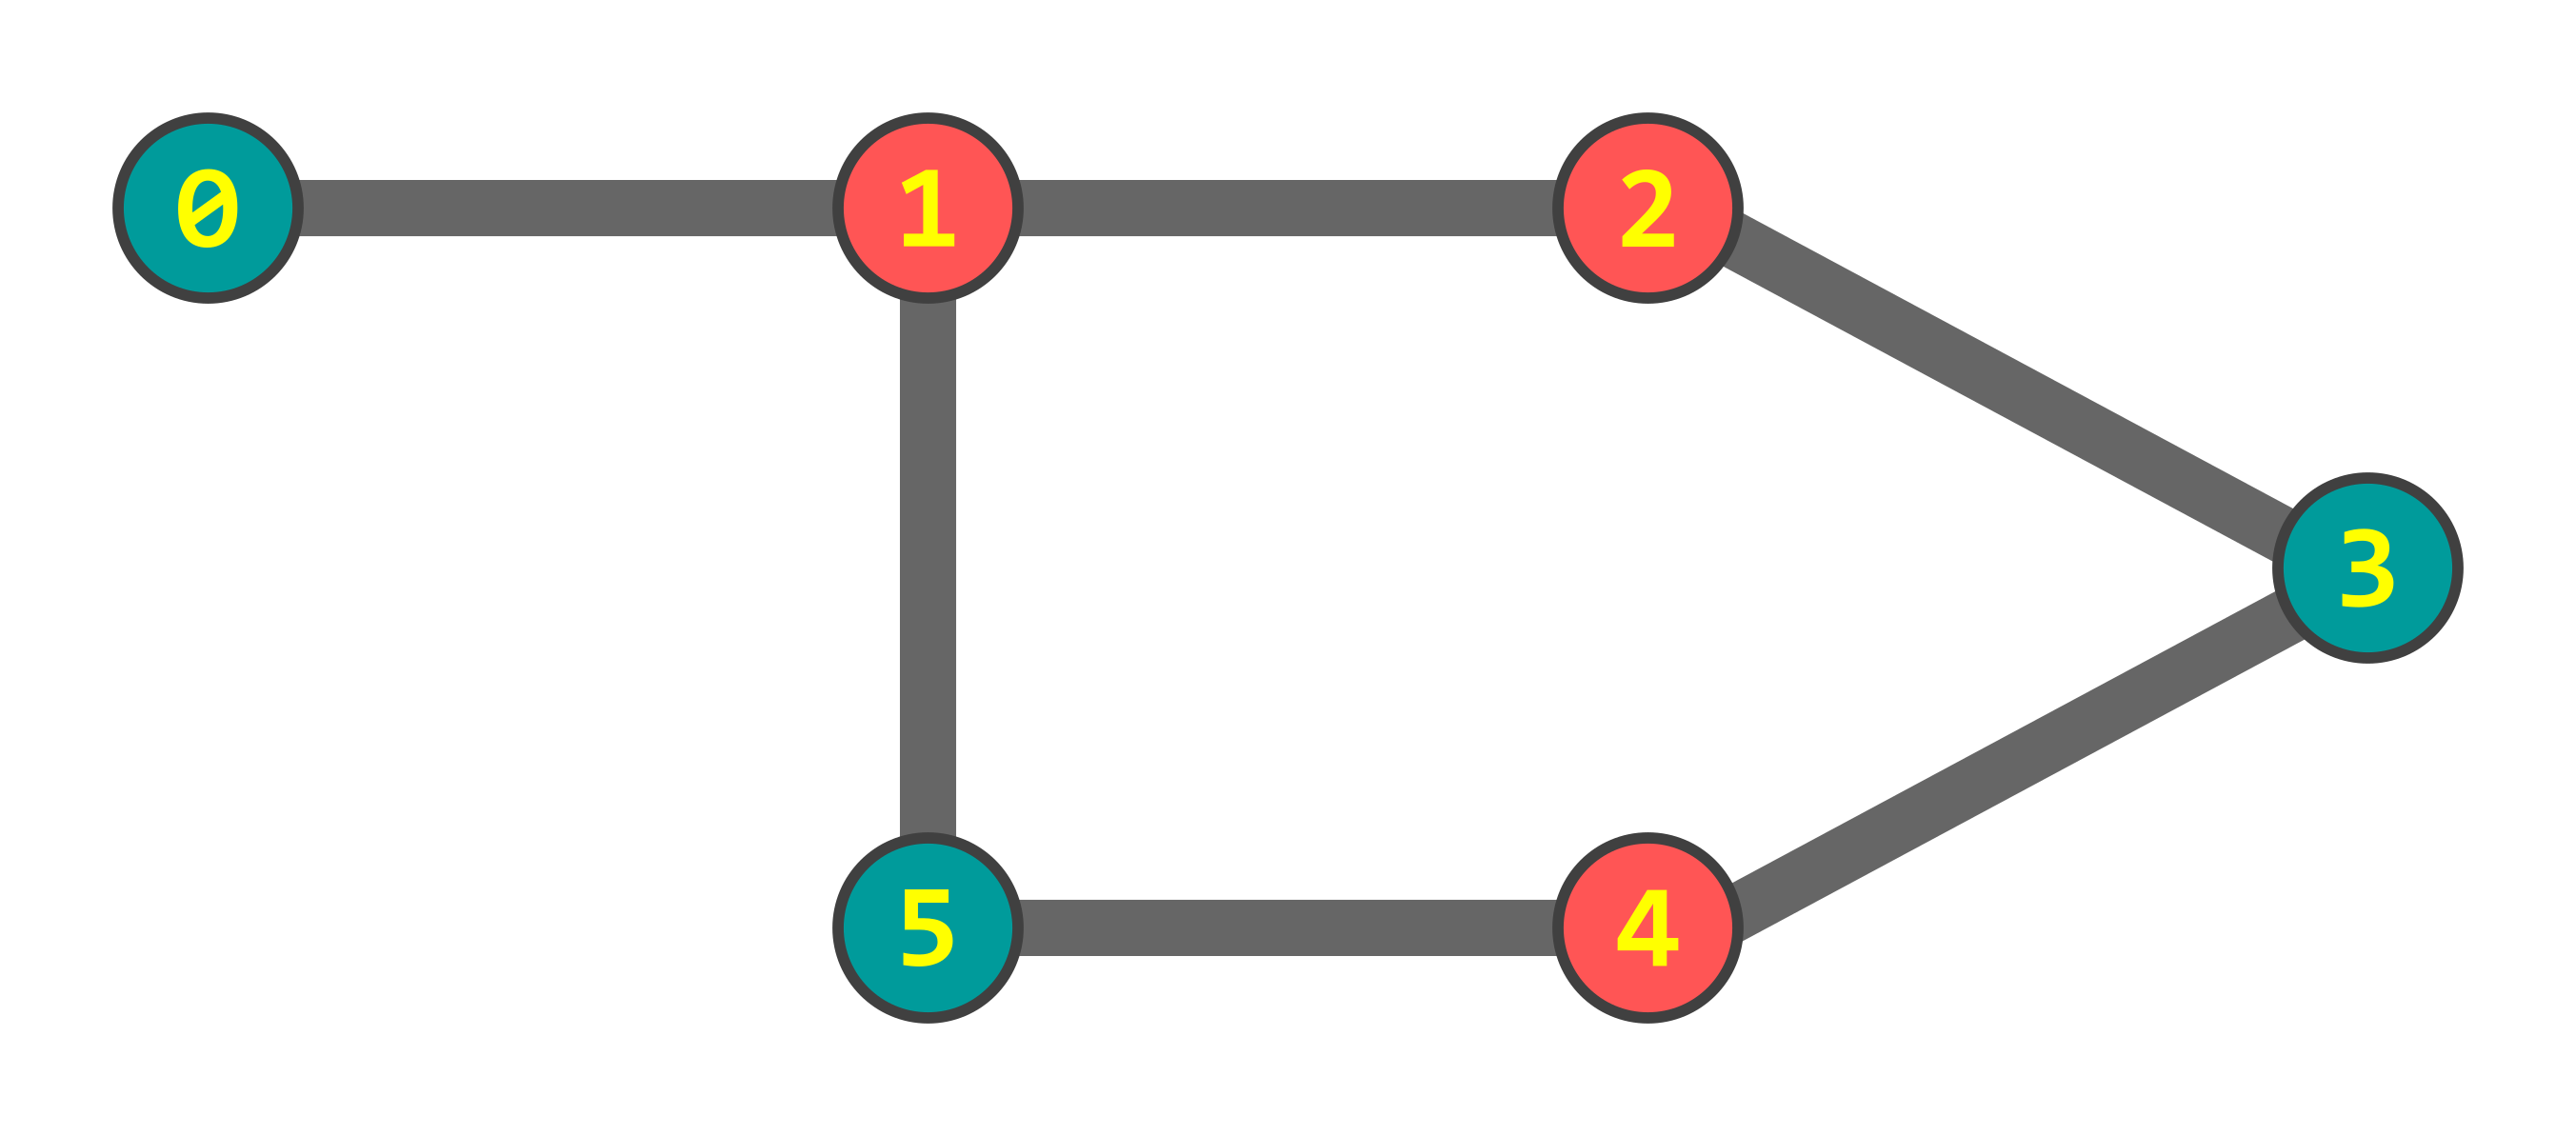
\includegraphics[width=0.9\linewidth,angle=0,origin=c]{out/ejB1.png}
    \caption{\label{ejB1} \textbf{Grafo original de ejemplo}}
\end{figure}

Para verlo podemos agregar un nodo para cada arista y unirlo a los vértices originales:
\begin{figure}[H]
    \centering
    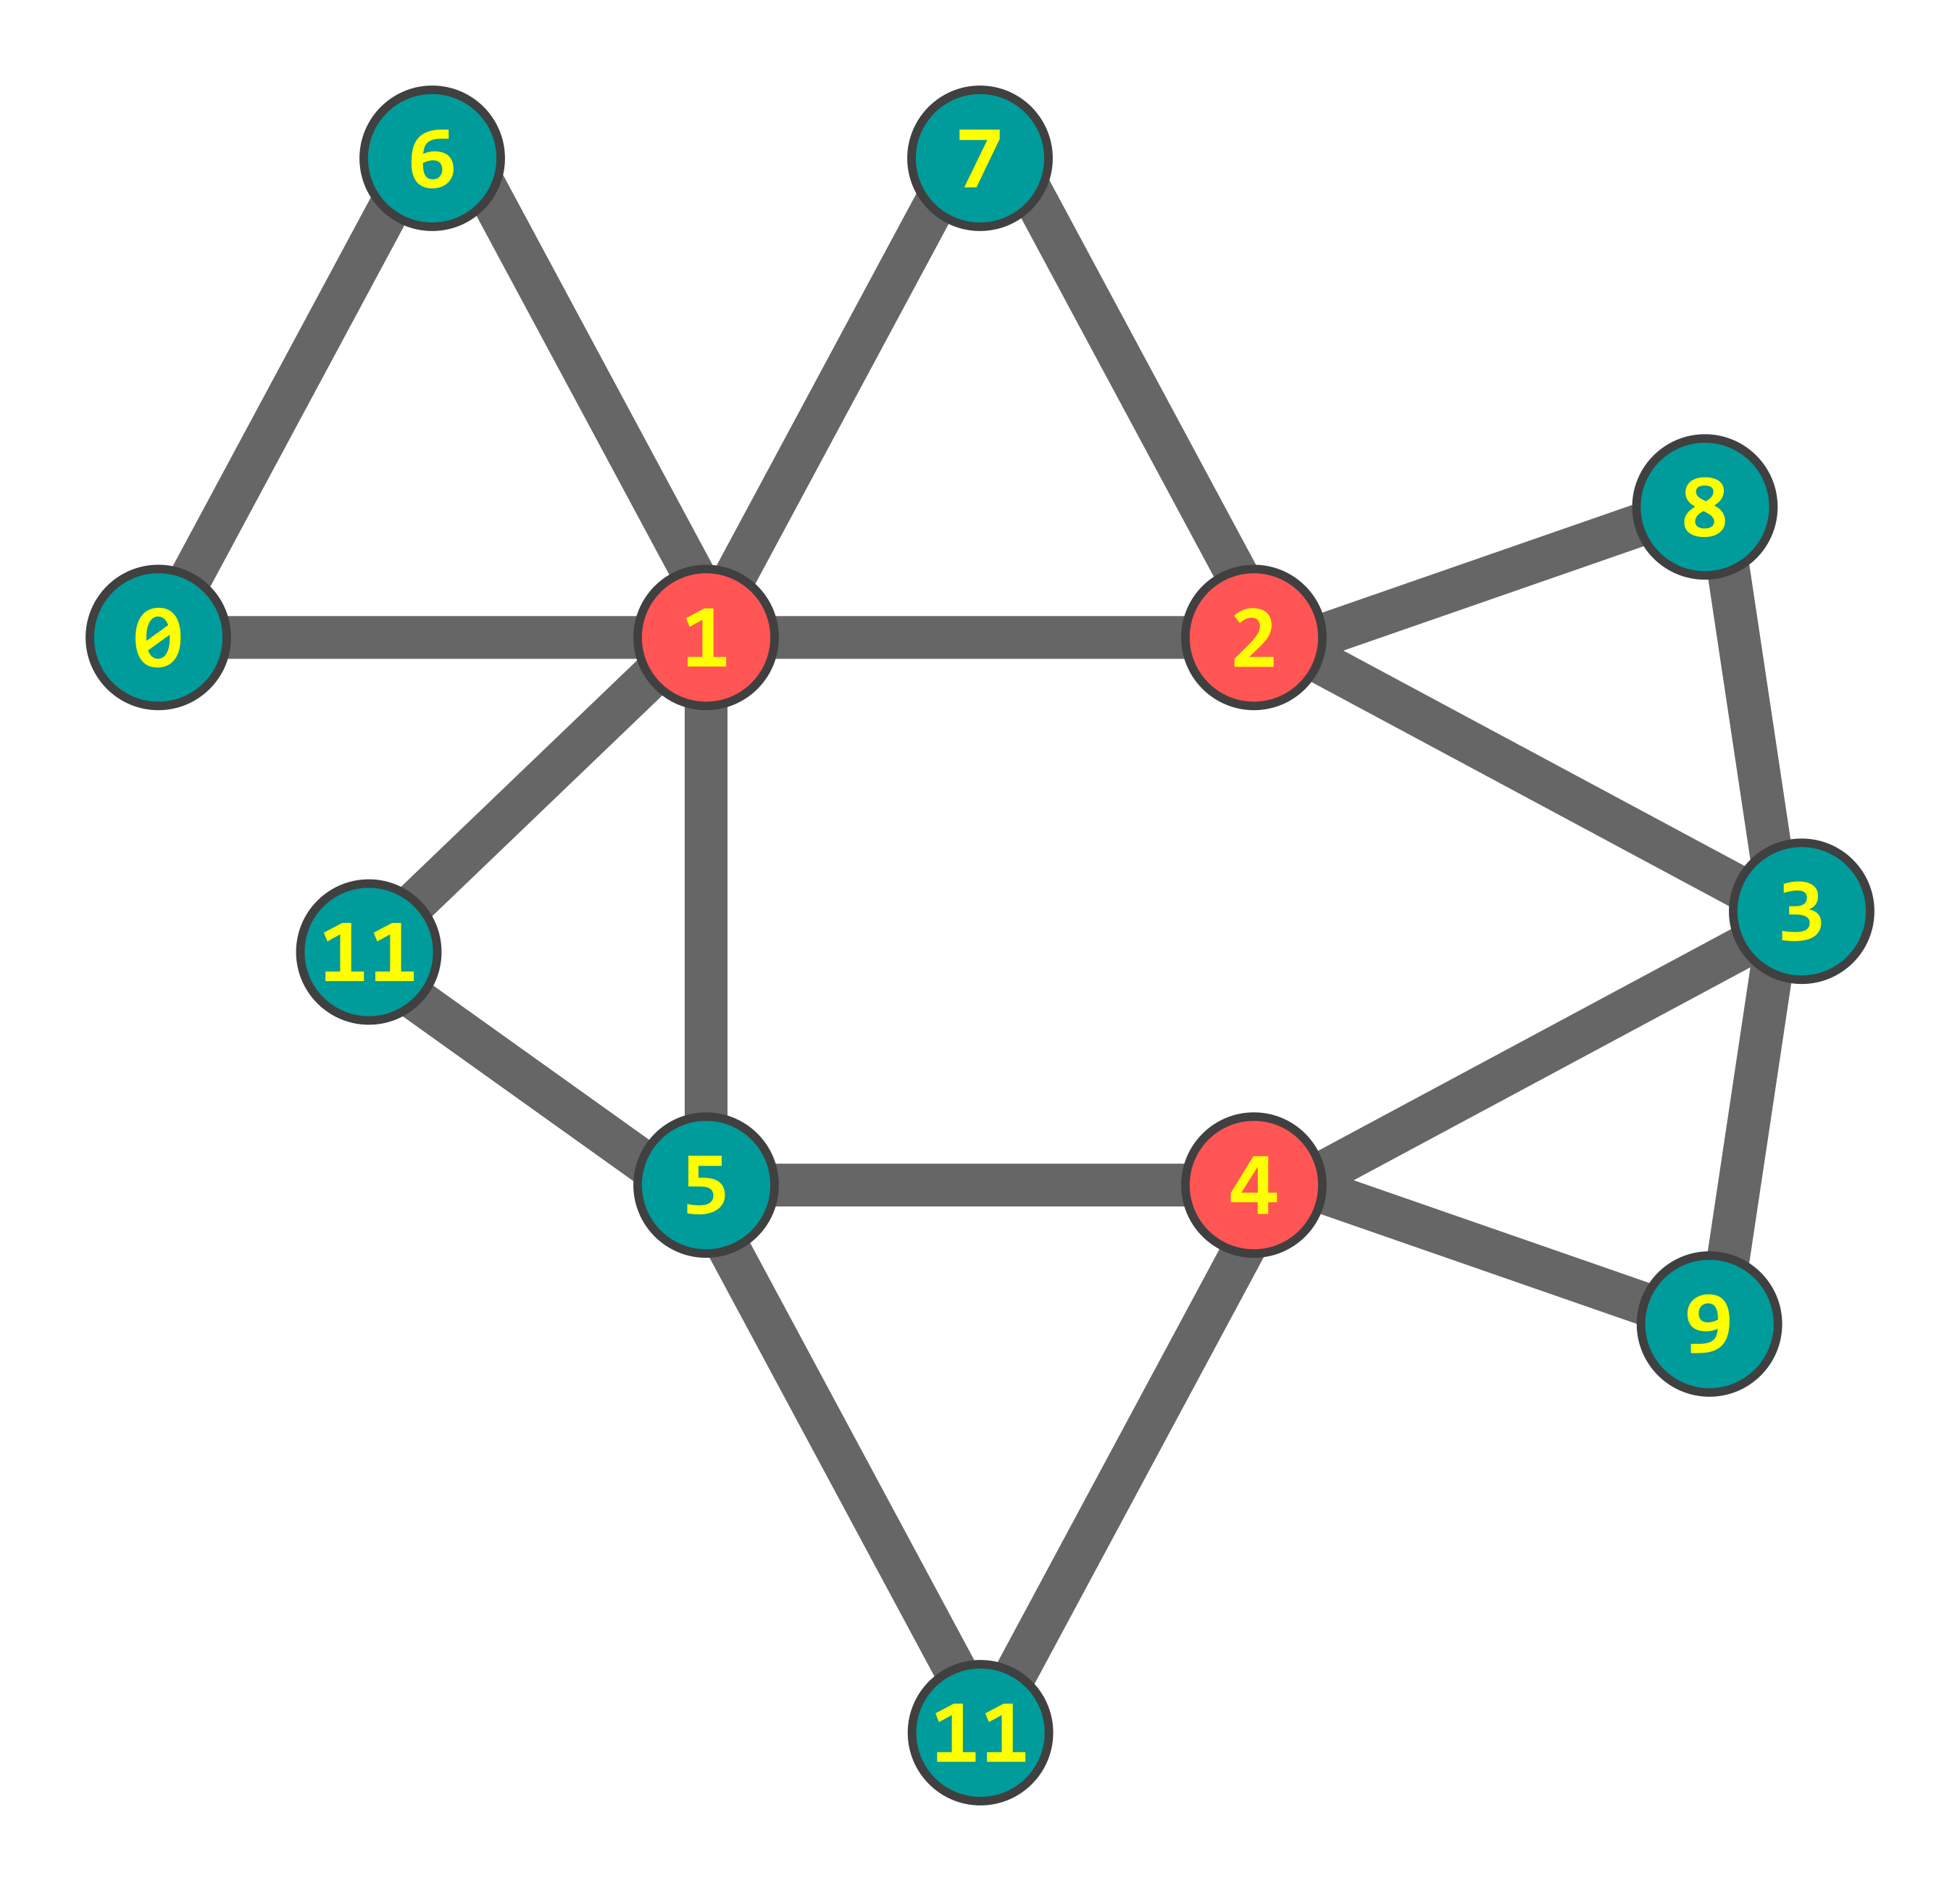
\includegraphics[width=0.9\linewidth,angle=0,origin=c]{out/ejB2.png}
    \caption{\label{ejB2} \textbf{Grafo transformado}. Nótese por ejemplo que se dada
    la arista $0\rightarrow 1$, se agrega \textcircled{6} unido a ambos.}
\end{figure}

Y como el set es un set dominante para el nuevo grafo, entonces el set es un vertex cover
para el grafo original.

% FIN DEL DOCUMENTO (SECCIÓN P2.2)
% NO BORRAR POR ACCIDENTE NI ESCRIBIR COSAS ABAJO
\end{document}